\chapter{Einführung}
\label{ch:01_introduction}

Die stilisierte Darstellung komplexer 3D-Szenen und der darin enthaltenen einzelnen Objekte mittels \ac{NPR} ist in der
modernen Computergrafik für technische und unterhaltende Anwendungen von großer Bedeutung.
Eine gezielte Stilisierung erhöht die visuelle Lesbarkeit, lenkt den Fokus des Betrachters und ermöglicht künstlerische
Abstraktionen (siehe~\ref{fig:borderlands_npr_example}).
Insbesondere bei großen Spieleproduktionen besteht die Notwendigkeit, wachsende Datenmengen und
Szenenkomplexitäten in Echtzeit bewältigen zu müssen~\cite[Abschn.~1]{magdicsPostprocessingNPREffects2013}.
Die effiziente Handhabung der resultierenden Performance-Engpässe erfordert hochskalierbare Rendering-Architekturen.
Die Gewährleistung dieser Skalierbarkeit erweist sich im Kontext der für \ac{NPR} oft erforderlichen Stil-Heterogenität
jedoch als komplexe Problemstellung und offenbart einen fundamentalen Konflikt innerhalb von
Standard-Rendering-Paradigmen, da diese strukturell für homogene Beleuchtungsberechnungen optimiert
sind~\cites[S.~34]{AdvancesRealTimeRendering}[Abschn.~20.1, S.~886--887]{akenine-mollerRealtimeRendering2019}.

\begin{figure}[htbp]
    \centering
    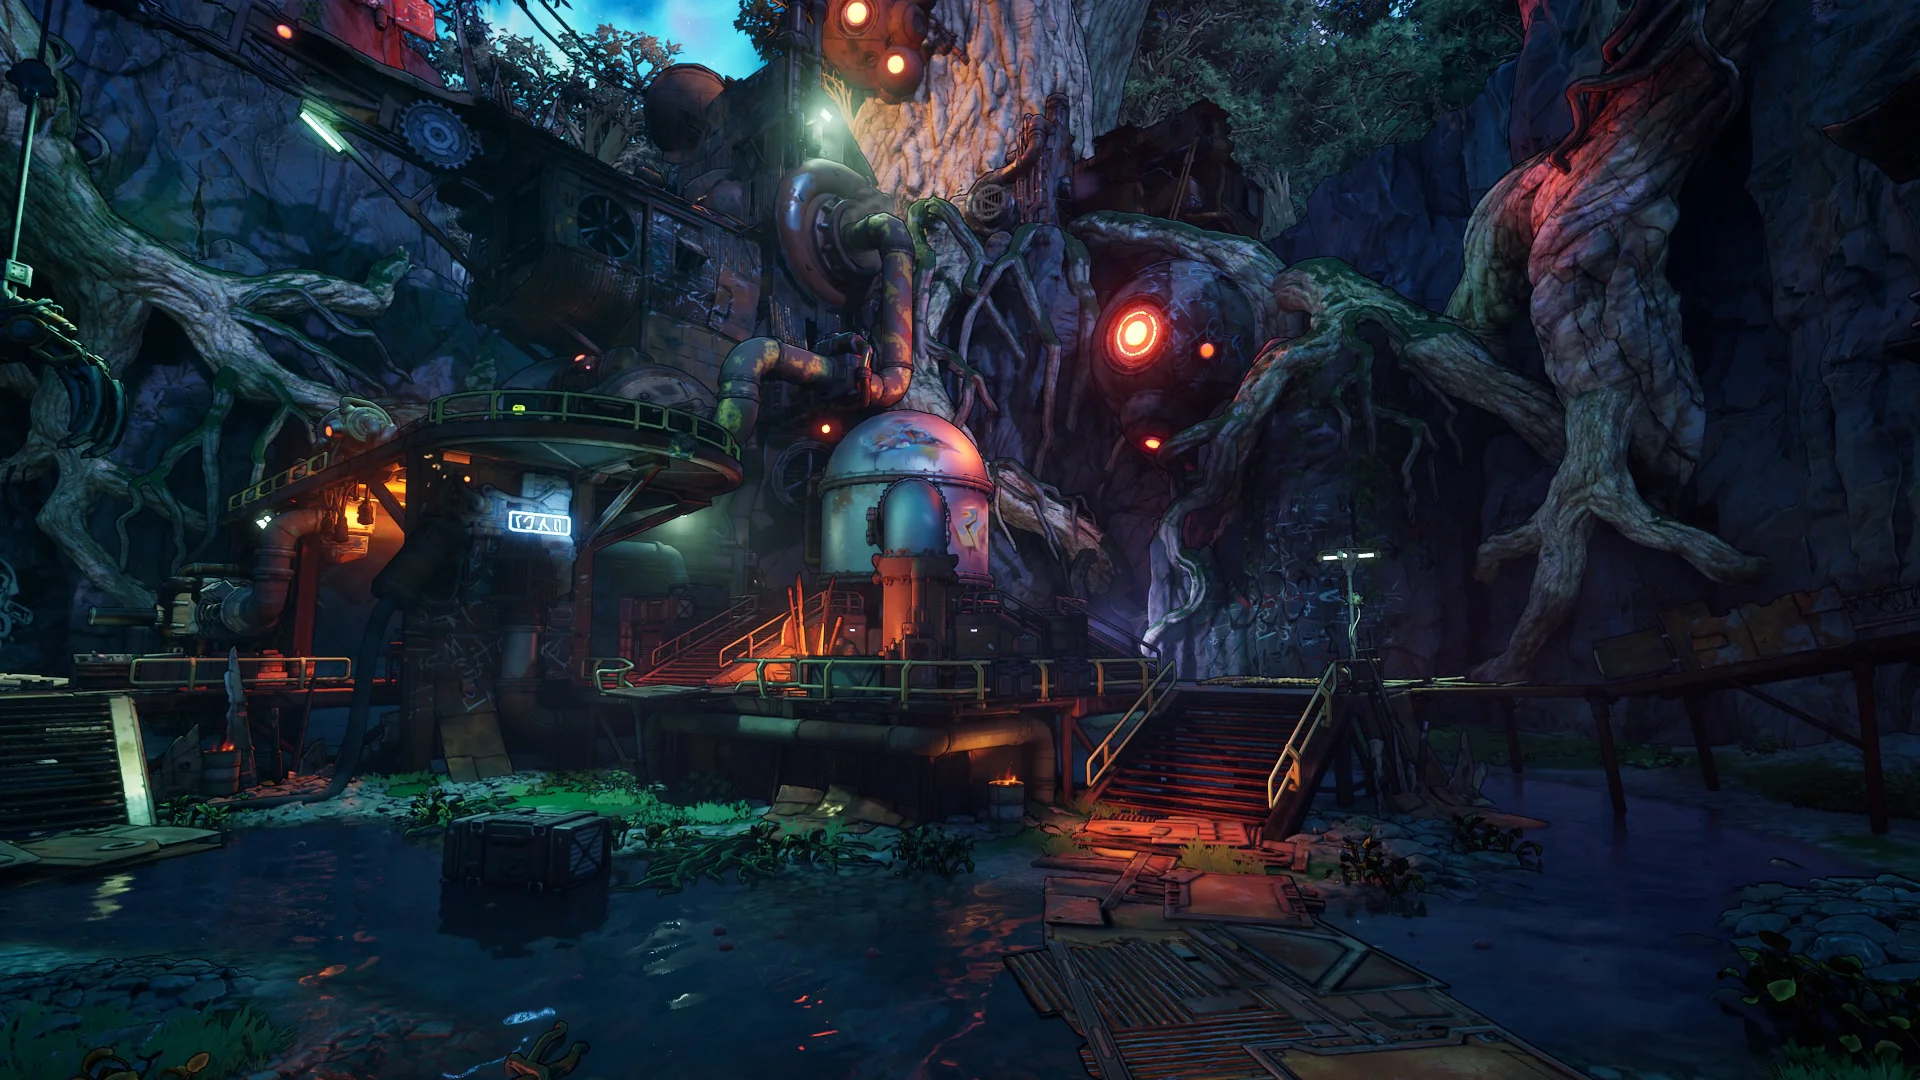
\includegraphics[width=0.85\textwidth]{abbildungen/Borderlands-4-Screenshot}
    \caption[Anwendungsbeispiel für Cel-Shading in \textit{Borderlands 4}]{Anwendungsbeispiel für künstlerisches NPR
    am Beispiel von \textit{Borderlands 4}
    (2025)~\cite{Borderlands4Screenshotsa}.}
    \label{fig:borderlands_npr_example}
\end{figure}


\section{Motivation \& Problemstellung}
\label{sec:0101_motivation_and_problem}

% Wirtschaftliche/Wissenschaftliche Relevanz von NPR.
\ac{NPR}-Effekte werden primär mit künstlerischen Umsetzungen und stilisierten Darstellungen in der
Unterhaltungsindustrie, wie etwa in Videospielen oder Filmproduktionen, in Verbindung gebracht.
Die gezielte Stilisierung ganzer Szenen oder einzelner Objekte zur Schaffung eines bestimmten künstlerischen Kontextes
bildet hierbei einen der Hauptanwendungszwecke von modernem
\ac{NPR}~\cite[S.651--652]{akenine-mollerRealtimeRendering2019}.
Darüber hinaus finden diese Techniken auch im Bereich von technischen Illustrationen, \ac{CAD}-Software oder
medizinischen Visualisierungen weitreichende Anwendung.
In diesen Fachbereichen erfüllt die Stilisierung oftmals den funktionalen Zweck, durch eine simplere oder abstraktere
Darstellung die allgemeine Lesbarkeit der Szene zu erhöhen oder den Fokus gezielt auf kritische Daten und spezifische
Elemente zu lenken~\cite[Abschn.~2]{goochNonphotorealisticLightingModel1998}.
Eine derartige funktionale Hervorhebung durch Simplifizierung ist mit gängigem \ac{PBR} in
dieser Form oft nicht möglich, da rein fotorealistische Ansätze visuell häufig zu detailreich
sind und die Wahrnehmbarkeit der wesentlichen Informationen
mindern~\cite[Abschn.~1]{magdicsPostprocessingNPREffects2013}.

% Status Quo Deferred Pipelines.
Moderne Echtzeit-Rendering-Pipelines müssen enorme Mengen an 3D-Geometriedaten verarbeiten und gleichzeitig hochkomplexe
Beleuchtungsszenarien aus zahlreichen Lichtquellen berechnen.
Das so genannte \textit{Deferred Rendering} entkoppelt die Geometrieverarbeitung strikt von der Lichtauswertung,
ermöglicht so die drastische Reduzierung des Rechenaufwandes in komplexen Szenarien und hat sich folglich als
Architektur-Paradigma zur effizienten Bewältigung hoher Lichtkomplexitäten etabliert.
Aufgrund ihres inhärenten Aufbaus weisen standard Deferred-Pipelines jedoch einen architektonischen Nachteil
auf, da sie in der Materialvielfalt (unterschiedliche Darstellungseigenschaften von Objekten) eingeschränkt sind.
Infolgedessen wurden Deferred-Paradigmen historisch primär für die Auswertung homogener,
fotorealistischer Oberflächen (\ac{PBR}) verwendet~\cite[Abschn.~1]{haradaForwardBringingDeferred2012}.

% Verlust der Semantik vs.~Granularität.
Deferred Rendering projiziert die dreidimensionale Szenengeometrie in einen zweidimensionalen \ac{G-Buffer}.
Bei dieser Überführung in den \textit{Screen-Space} gehen die Identität der Objekte und diverse semantische
Informationen verloren.
Stattdessen werden in klassischen Pipelines lediglich physikalische Oberflächendaten für standardisierte
Lichtberechnungen (\ac{PBR}), wie etwa Albedo, Normalen oder Rauheit, gespeichert.
Viele \ac{NPR}-Effekte erfordern für eine fehlerfreie Ausführung jedoch zwingend einen gewissen Grad an semantischen
Informationen~\cite[Abschn.~2.1 u.~3.3.2]{fonsecaDeferredShadingTutorial}.
Die Zuweisung verschiedener Zeichenstile wie \textit{Toon-Shading} oder die exakte Trennung überlappender
Objekte durch Umrisslinien benötigen beispielsweise spezifische Material-Identifikatoren (\textit{Shading-Model-IDs}),
oder Objekt-IDs~\cites[Kap.~15.2.3]{akenine-mollerRealtimeRendering2019}
[Folie~\textit{Our GBuffer Layout}]{gameworksToonRenderingHiFi}.
Diese Metadaten fehlen in einem klassischen, auf \ac{PBR}-optimierten \ac{G-Buffer}.
Dieser Umstand führt dazu, dass \ac{NPR} in Deferred-Architekturen häufig zu einem rein
globalen Post-Processing-Filter über das gesamte Bild reduziert
wird~\cite[Abschn.~1]{magdicsPostprocessingNPREffects2013}.
Eine granulare, selektive/hybride Stilisierung, z.~B.\ Bauteil A als Skizze, Bauteil B massiv schattiert, wird dadurch technisch
erschwert.
Bei hoher stilistischer Vielfalt und stark selektiven Anwendungsfällen wird daher oft auf klassisches
\textit{Forward-Rendering} zurückgegriffen, in welchem Objekte einzeln ausgewertet werden und so den Großteil ihrer
semantischen Informationen im Rendering-Prozess behalten.
Dies erweist sich wiederum als ineffizient bei hoher
Beleuchtungskomplexität~\cite[Abschn.~1]{haradaForwardBringingDeferred2012}.

% überleitung und Hardware-Restriktionen.
Die Kombination aus massenhafter Geometrie, Beleuchtungskomplexität und stilistischer Vielfalt zwingt in der Praxis
die Basis-Rendering-Paradigmen wie klassisches Forward oder Deferred an ihre individuellen hardwaretechnischen
Leistungsgrenzen.
Die Industrie greift hier auf diverse individuelle Lösungsansätze und Vermischungen von Rendering-Paradigmen zurück
(siehe Kap.~\ref{sec:0302_industry_state}).
Dabei offenbart sich ein grundlegender architektonischer Konflikt: Architekturen leiden bei der Stilisierung vieler
Objekte entweder unter massiven redundanten Zeichenoperationen bei überlappender
Geometrie~\cite[Abschn.~1]{fatahalianReducingShadingGPUs2010}, oder die Auswertung der diversen Stildaten
überlastet die Speicher- und Rechenkapazitäten der
Grafikhardware~\cite[Abschn.~6]{schiedDeferredAttributeInterpolation2015}.
In der Praxis mangelt es an empirischen Werkzeugen sowie einer systematischen Dokumentation der Bedingungen,
unter denen diese Leistungseinbrüche beim selektiven \ac{NPR} auftreten.
Daraus leitet sich das Ziel dieser Arbeit ab.


\section{Ziel der Arbeit \& Forschungsfrage}
\label{sec:0102_goal_and_core_question}

% Das primäre Ziel (WHAT & WHY).
Das Ziel dieser Arbeit ist die Entwicklung eines Praxiswerkzeugs zur empirischen Performance-Analyse
verschiedener Basis-Rendering-Architekturen im Kontext des selektiven \ac{NPR}.
Aus den gewonnenen Messdaten wird ein heuristisches Entscheidungsmodell abgeleitet, das als Orientierungshilfe
für die Evaluation elementarer Rendering-Paradigmen dient.
Die untersuchten Basis-Pipelines umfassen dabei ein Single-Pass-Forward-Rendering als Referenz, ein
Single-Pass-Deferred-Rendering mit einer monolithischen Shader-Struktur sowie einen Multi-Pass-Deferred-Ansatz mit
volumetrischer Lichtauswertung (\textit{Light Volumes}).
Das Evaluations-Framework sowie das resultierende Modell bieten Entwicklern, auch ohne tiefgehende
Spezialisierung in der Grafikprogrammierung, eine objektive Entscheidungsgrundlage, um anhand der
Szenen- und Stilkomplexität die passende Basis-Architektur zu wählen, bevor Performance-Engpässe entstehen.
Zusätzlich dient die Software als isolierte Referenzumgebung, um die Leistungsgrenzen dieser
Rendering-Paradigmen unabhängig zu quantifizieren.

% Forschungsfrage.
Aus diesen Zielen leitet sich die zentrale Forschungsfrage der vorliegenden Arbeit ab, die im Rahmen der Systemanalyse
empirisch untersucht und beantwortet wird:
\begin{quote}
    \textit{Wie lassen sich Non-Photorealistic Rendering-Pipelines architektonisch so konzipieren und umsetzen, dass
    eine selektive, objektbasierte Stilisierung unter hoher Entropie ermöglicht wird, und wie verhält
    sich dabei die Gesamteffizienz der Pipeline im Vergleich zur Szenenkomplexität? Welche Aspekte bilden hier die
    individuellen Performance-Engpässe und Limitierungen und wie verschieben sich diese zwischen den verschiedenen
    Rendering-Pipelines?}
\end{quote}

% Methodik und Artefakt (HOW).
Als zentrales Software-Artefakt wird das C++/OpenGL-basierte Framework \textquote{\ac{HyDra}} realisiert,
welches die drei Basis-Pipelines isoliert umsetzt.
Es stellt den Kern dieser Arbeit dar und dient als kontrollierte Testumgebung zur Generierung deterministischer
Messreihen für die Beantwortung der Forschungsfragen.

% Thematische Eingrenzung.
Komplexe Sondereffekte, wie die Verarbeitung semitransparenter Geometrie, \textit{Anti-Aliasing} oder
erweiterte Lichtmodelle (neben einfachen Punktlichtern), sind nicht Gegenstand dieser Arbeit.
Eine Berücksichtigung dieser Effekte würde zusätzliche Störfaktoren einführen und den Fokus von der
isolierten Evaluation der Basis-Rendering-Architekturen ablenken.


\section{Nutzung Generativer KI}
\label{sec:0103_AI}

Im Rahmen der Erstellung dieser Ausarbeitung wurden generative KI-Werkzeuge verwendet und als unterstützende Hilfsmittel
herangezogen, namentlich \textit{Google-Antigravity} und \textit{Google-Gemini}.
Diese Systeme wurden primär zur methodischen Strukturierung einzelner Kapitel, zur Erstellung von
UML-Aktivitätsdiagrammen in LaTeX, zur erweiterten Recherche, zur Code-Analyse bei der Fehlerbehandlung sowie
für die Generierung von Boilerplate-Code und Python-Skripten für die Visualisierung der Benchmark-Rohdaten eingesetzt.
Gemäß den Vorgaben de §14a der Rahmenprüfungsordnung sind die vollständigen, inhaltlich relevanten Chat-Verläufe,
bestehend aus den verwendeten Prompts und den generierten Antworten der KI-Modelle, im digitalen Anhang dieser Arbeit
dokumentiert.


\section{Aufbau der Arbeit}
\label{sec:0104_setup}

% Aufbau.
Die vorliegende Arbeit gliedert sich wie folgt:
Kapitel~\ref{ch:02_grundlagen} vermittelt zunächst die architektonischen und hardwaretechnischen Grundlagen sowie
relevante technische Begrifflichkeiten, die für das Verständnis der weiteren Untersuchungen erforderlich sind.
Kapitel~\ref{ch:03_acedemic_and_industry_state} analysiert den aktuellen Stand der Forschung sowie der Industriepraxis
und grenzt darauf aufbauend die bestehende Forschungslücke ab.
Kapitel~\ref{ch:04_konzeption_realisierung} dokumentiert die Konzeption und softwaretechnische Realisierung des
entwickelten
Evaluations-Frameworks sowie etwaige praktische und architektonische Grenzen der verschiedenen
Rendering-Architekturen.
Kapitel~\ref{ch:05_evaluation} präsentiert die Methodik der durchgeführten Versuchsreihen und wertet die
empirischen Messdaten der untersuchten Rendering-Pipelines aus.
Kapitel~\ref{ch:06_diskussion} und Kapitel~\ref{ch:07_zusammenfassung_ausblick} führen die gewonnenen Erkenntnisse
abschließend in einem heuristischen Entscheidungsmodell zusammen, diskutieren die Limitationen der Arbeit und
schließen diese mit einem Ausblick auf künftige Forschungsmöglichkeiten und Erweiterungen der Evaluationssoftware ab.